\documentclass[10pt]{article}
\usepackage[paperwidth=11.8cm,paperheight=4.5cm,margin=0pt]{geometry}
\usepackage{amsmath,amssymb}
\usepackage{mathptmx}
\renewcommand{\hbar}{\mathchar'26\mkern-9mu h}
\usepackage{tikz}
\pagestyle{empty}
\begin{document}
\special{papersize=11.8cm,4.5cm}
\noindent
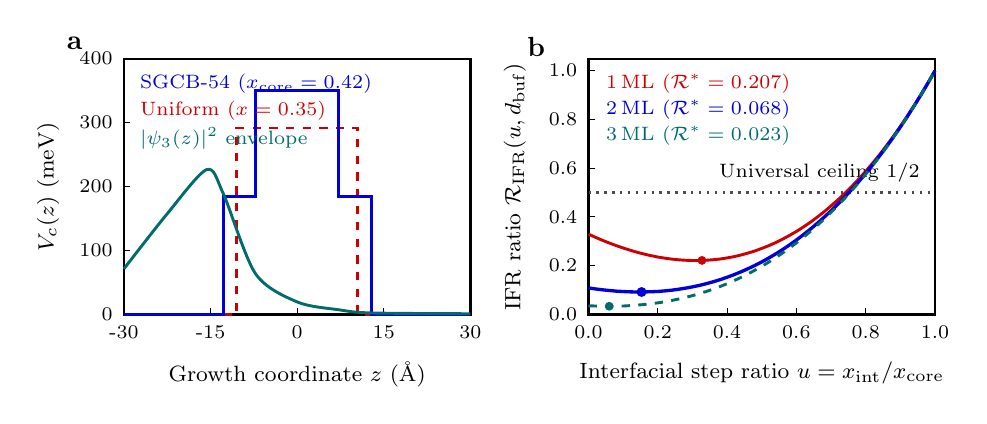
\begin{tikzpicture}[x=1cm,y=1cm,font=\footnotesize]
  % Panel a: Conduction band & envelope probability
  \node[anchor=north west,font=\bfseries\normalsize] at (0.10,4.35) {a};
  \draw[thick] (0.95,0.70) rectangle (5.35,3.95);
  \foreach \v/\y in {0/0.70, 100/1.51, 200/2.33, 300/3.14, 400/3.95} {
    \draw (0.95,\y) -- (1.03,\y);
    \node[left,font=\scriptsize] at (0.93,\y) {\v};
  }
  \foreach \xval/\xpos in {-30/0.95, -15/2.05, 0/3.15, 15/4.25, 30/5.35} {
    \draw (\xpos,0.70) -- (\xpos,0.78);
    \node[below,font=\scriptsize] at (\xpos,0.68) {\xval};
  }
  \node[below,font=\footnotesize] at (3.15,0.22) {Growth coordinate $z$ (\AA)};
  \node[rotate=90,above,font=\footnotesize] at (0.25,2.32) {$V_c(z)$ (meV)};

  \draw[dashed,red!80!black,line width=0.95pt]
    (0.95,0.70) -- (2.38,0.70) -- (2.38,3.07) -- (3.92,3.07) -- (3.92,0.70) -- (5.35,0.70);
  \draw[blue!85!black,line width=1.15pt]
    (0.95,0.70) -- (2.21,0.70) -- (2.21,2.20) -- (2.62,2.20) -- (2.62,3.55) -- (3.68,3.55) -- (3.68,2.20) -- (4.09,2.20) -- (4.09,0.70) -- (5.35,0.70);
  \draw[teal!85!black,line width=1.05pt,smooth]
    plot coordinates {(0.95,1.28) (1.50,1.98) (2.00,2.54) (2.21,2.24) (2.62,1.22) (3.15,0.86) (3.68,0.76) (4.09,0.72) (5.35,0.71)};

  \node[anchor=north west,font=\scriptsize,blue!85!black] at (1.03,3.88) {SGCB-54 ($x_{\mathrm{core}}=0.42$)};
  \node[anchor=north west,font=\scriptsize,red!80!black] at (1.03,3.54) {Uniform ($x=0.35$)};
  \node[anchor=north west,font=\scriptsize,teal!85!black] at (1.03,3.20) {$|\psi_3(z)|^2$ envelope};

  % Panel b: Theorem 1 R_IFR(u, d_buf)
  \node[anchor=north west,font=\bfseries\normalsize] at (5.95,4.35) {b};
  \draw[thick] (6.85,0.70) rectangle (11.25,3.95);
  \foreach \v/\y in {0.0/0.70, 0.2/1.32, 0.4/1.94, 0.6/2.56, 0.8/3.18, 1.0/3.80} {
    \draw (6.85,\y) -- (6.93,\y);
    \node[left,font=\scriptsize] at (6.83,\y) {\v};
  }
  \foreach \uval/\xpos in {0.0/6.85, 0.2/7.73, 0.4/8.61, 0.6/9.49, 0.8/10.37, 1.0/11.25} {
    \draw (\xpos,0.70) -- (\xpos,0.78);
    \node[below,font=\scriptsize] at (\xpos,0.68) {\uval};
  }
  \node[below,font=\footnotesize] at (9.05,0.22) {Interfacial step ratio $u = x_{\mathrm{int}}/x_{\mathrm{core}}$};
  \node[rotate=90,above,font=\footnotesize] at (6.18,2.32) {IFR ratio $\mathcal{R}_{\mathrm{IFR}}(u,d_{\mathrm{buf}})$};

  \draw[dotted,black!70,line width=0.85pt] (6.85,2.25) -- (11.25,2.25);
  \node[anchor=south east,font=\scriptsize] at (11.18,2.26) {Universal ceiling $1/2$};

  \draw[red!80!black,line width=1.05pt] (6.850,1.721) -- (6.938,1.681) -- (7.026,1.643) -- (7.114,1.608) -- (7.202,1.575) -- (7.290,1.545) -- (7.378,1.517) -- (7.466,1.491) -- (7.554,1.468) -- (7.642,1.448) -- (7.730,1.430) -- (7.818,1.416) -- (7.906,1.404) -- (7.994,1.395) -- (8.082,1.389) -- (8.170,1.386) -- (8.258,1.386) -- (8.346,1.389) -- (8.434,1.396) -- (8.522,1.405) -- (8.610,1.419) -- (8.698,1.435) -- (8.786,1.456) -- (8.874,1.480) -- (8.962,1.507) -- (9.050,1.539) -- (9.138,1.574) -- (9.226,1.613) -- (9.314,1.657) -- (9.402,1.704) -- (9.490,1.755) -- (9.578,1.811) -- (9.666,1.871) -- (9.754,1.936) -- (9.842,2.005) -- (9.930,2.079) -- (10.018,2.157) -- (10.106,2.240) -- (10.194,2.328) -- (10.282,2.421) -- (10.370,2.519) -- (10.458,2.622) -- (10.546,2.730) -- (10.634,2.844) -- (10.722,2.963) -- (10.810,3.087) -- (10.898,3.217) -- (10.986,3.353) -- (11.074,3.494) -- (11.162,3.642) -- (11.250,3.795);
  \draw[blue!85!black,line width=1.2pt] (6.850,1.038) -- (6.938,1.025) -- (7.026,1.014) -- (7.114,1.005) -- (7.202,0.997) -- (7.290,0.992) -- (7.378,0.988) -- (7.466,0.986) -- (7.554,0.987) -- (7.642,0.989) -- (7.730,0.993) -- (7.818,1.000) -- (7.906,1.009) -- (7.994,1.021) -- (8.082,1.035) -- (8.170,1.051) -- (8.258,1.070) -- (8.346,1.092) -- (8.434,1.116) -- (8.522,1.143) -- (8.610,1.173) -- (8.698,1.206) -- (8.786,1.242) -- (8.874,1.281) -- (8.962,1.323) -- (9.050,1.368) -- (9.138,1.417) -- (9.226,1.469) -- (9.314,1.524) -- (9.402,1.583) -- (9.490,1.646) -- (9.578,1.713) -- (9.666,1.783) -- (9.754,1.857) -- (9.842,1.935) -- (9.930,2.017) -- (10.018,2.103) -- (10.106,2.194) -- (10.194,2.289) -- (10.282,2.388) -- (10.370,2.491) -- (10.458,2.600) -- (10.546,2.713) -- (10.634,2.830) -- (10.722,2.953) -- (10.810,3.080) -- (10.898,3.213) -- (10.986,3.351) -- (11.074,3.493) -- (11.162,3.642) -- (11.250,3.795);
  \draw[teal!85!black,line width=1.05pt,dashed] (6.850,0.811) -- (6.938,0.808) -- (7.026,0.805) -- (7.114,0.805) -- (7.202,0.806) -- (7.290,0.808) -- (7.378,0.813) -- (7.466,0.819) -- (7.554,0.827) -- (7.642,0.837) -- (7.730,0.848) -- (7.818,0.862) -- (7.906,0.878) -- (7.994,0.897) -- (8.082,0.917) -- (8.170,0.940) -- (8.258,0.965) -- (8.346,0.993) -- (8.434,1.023) -- (8.522,1.056) -- (8.610,1.091) -- (8.698,1.130) -- (8.786,1.171) -- (8.874,1.215) -- (8.962,1.262) -- (9.050,1.311) -- (9.138,1.365) -- (9.226,1.421) -- (9.314,1.481) -- (9.402,1.544) -- (9.490,1.610) -- (9.578,1.680) -- (9.666,1.753) -- (9.754,1.831) -- (9.842,1.912) -- (9.930,1.997) -- (10.018,2.086) -- (10.106,2.179) -- (10.194,2.276) -- (10.282,2.377) -- (10.370,2.482) -- (10.458,2.592) -- (10.546,2.707) -- (10.634,2.826) -- (10.722,2.950) -- (10.810,3.078) -- (10.898,3.211) -- (10.986,3.350) -- (11.074,3.493) -- (11.162,3.642) -- (11.250,3.795);
  \fill[red!80!black] (8.291,1.387) circle (1.6pt);
  \fill[blue!85!black] (7.524,0.986) circle (1.8pt);
  \fill[teal!85!black] (7.113,0.805) circle (1.6pt);

  \node[anchor=north west,font=\scriptsize,red!80!black] at (6.95,3.88) {$1\,\mathrm{ML}$ ($\mathcal{R}^*=0.207$)};
  \node[anchor=north west,font=\scriptsize,blue!85!black] at (6.95,3.55) {$2\,\mathrm{ML}$ ($\mathcal{R}^*=0.068$)};
  \node[anchor=north west,font=\scriptsize,teal!85!black] at (6.95,3.22) {$3\,\mathrm{ML}$ ($\mathcal{R}^*=0.023$)};
\end{tikzpicture}
\end{document}
